\begin{ex}
	Cách nào sau đây dùng để xác định nhiệt độ trong thang nhiệt độ Celsius?
	\choice
	{Lấy nhiệt độ của nước khi đóng băng $\left(10^\circ C\right)$ và nhiệt độ sôi của nước $\left(100^\circ C\right)$ làm chuẩn}
	{Lấy nhiệt độ của nước khi đóng băng $\left(100^\circ C\right)$ và nhiệt độ sôi của nước $\left(0^\circ C\right)$ làm chuẩn}
	{\True Lấy nhiệt độ của nước khi đóng băng $\left(0^\circ C\right)$ và nhiệt độ sôi của nước $\left(100^\circ C\right)$ làm chuẩn}
	{Lấy nhiệt độ của nước khi đóng băng $\left(100^\circ C\right)$ và nhiệt độ sôi của nước $\left(10^\circ C\right)$ làm chuẩn}
	\loigiai{
		Thang nhiệt độ Celsius được định nghĩa bằng cách lấy hai điểm cố định là nhiệt độ đóng băng của nước ($0^\circ C$) và nhiệt độ sôi của nước ($100^\circ C$) ở 1 atm làm chuẩn.
	}
	\haidong{2}
\end{ex}
\begin{ex}
	Biểu thức nào sau đây gần đúng khi biến đổi nhiệt độ từ thang Celsius sang thang Kelvin?
	\choice
	{$T(K)\approx t\left(^\circ C\right)-273$}
	{\True $T(K)\approx t\left(^\circ C\right)+273$}
	{$T(K)\approx \dfrac{t\left(^\circ C\right)+273}{2}$}
	{$T(K)\approx 2 t\left(^\circ C\right)+273$}
	\loigiai{
		Công thức chính xác để chuyển đổi từ nhiệt độ Celsius sang nhiệt độ Kelvin là $T(K)=t\left(^\circ C\right) + 273$.
	}
	\haidong{3}\end{ex}
	\begin{ex}
		"Độ không tuyệt đối" là nhiệt độ ứng với
		\choice
		{\True $0 \ K$}
		{$0^\circ C$}
		{$273^\circ C$}
		{$273 \ K$}
		\loigiai{
			"Độ không tuyệt đối" ứng với nhiệt độ $0 \ K$, nơi mà các phân tử ngừng chuyển động nhiệt hoàn toàn.
		}
		\haidong{2}\end{ex}
		\begin{ex}
			Nhiệt kế chất lỏng được chế tạo dựa trên nguyên tắc nào?
			\choice
			{\True Sự nở vì nhiệt của chất lỏng}
			{Sự nở ra của chất lỏng khi nhiệt độ giảm}
			{Sự co lại của chất lỏng khi nhiệt độ tăng}
			{Sự nở của chất lỏng không phụ thuộc vào nhiệt độ}
			\loigiai{
				Nhiệt kế chất lỏng được chế tạo dựa trên nguyên tắc sự nở vì nhiệt của chất lỏng. Khi nhiệt độ thay đổi, thể tích của chất lỏng trong nhiệt kế sẽ thay đổi tương ứng.
			}
			\haidong{2}\end{ex}
			\begin{ex}
				Không thể dùng nhiệt kế rượu để đo nhiệt độ của hơi nước đang sôi vì
				\choice
				{rượu sôi ở nhiệt độ cao hơn $100^\circ C$}
				{\True rượu sôi ở nhiệt độ thấp hơn $100^\circ C$}
				{rượu đông đặc ở nhiệt độ thấp hơn $100^\circ C$}
				{rượu đông đặc ở nhiệt độ thấp hơn $0^\circ C$} 
				\loigiai{
					Không thể dùng nhiệt kế rượu để đo nhiệt độ của hơi nước đang sôi vì rượu sôi ở nhiệt độ thấp hơn $100^\circ C$, do đó nó sẽ bốc hơi trước khi đo được nhiệt độ này.
				}
				\haidong{2}\end{ex}
				\begin{ex}
					Nhiệt độ đông đặc của rượu là $-117^\circ C$, của thủy ngân là $-38,83^\circ C$. Ở các nước lạnh người ta 
						\immini{\choice
						{dùng nhiệt kế thủy ngân vì nhiệt kế thủy ngân rất chính xác}
						{dùng nhiệt kế thủy ngân vì nhiệt độ đông đặc của thủy ngân cao hơn nhiệt độ đông đặc của rượu}
						{dùng nhiệt kế thủy ngân vì ở âm vài chục $^\circ C$ rượu bay hơi hết}
						{\True dùng nhiệt kế rượu vì nhiệt kế rượu có thể đo nhiệt độ môi trường $-50^\circ C$}}
					{		\vspace*{1 cm} 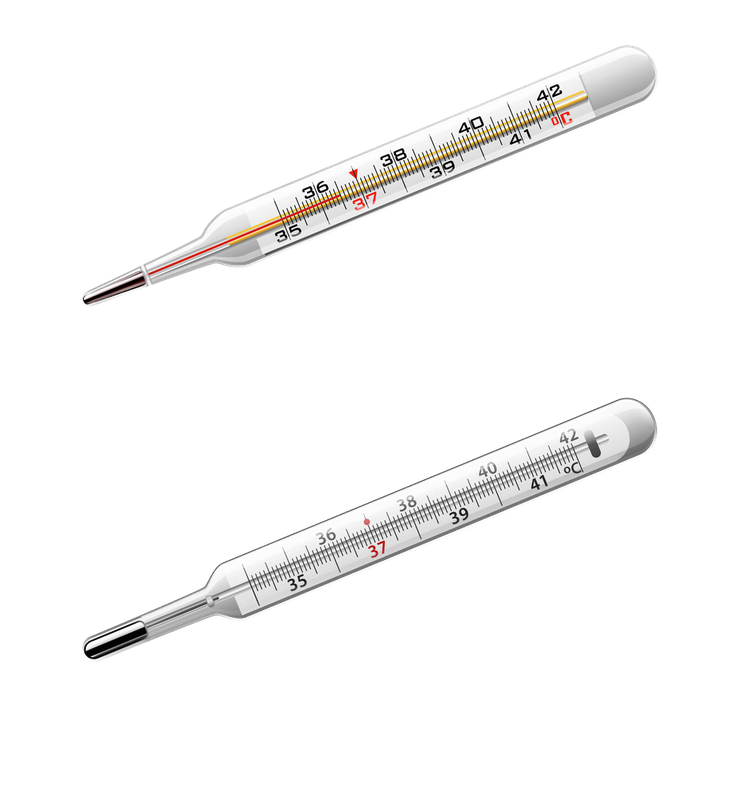
\includegraphics[width=4cm]{Images/nhietkeruou}
					}
					\loigiai{
						Vì nhiệt độ đông đặc của rượu thấp hơn nhiều so với thủy ngân (rượu: $-117^\circ C$, thủy ngân: $-38,83^\circ C$) nên ở các nước lạnh, nơi nhiệt độ có thể xuống thấp đến $-50^\circ C$, người ta dùng nhiệt kế rượu để đo nhiệt độ.
					}
					\haidong{2}\end{ex}
					\begin{ex}
	Người ta cho hai vật dẫn nhiệt A và B tiếp xúc với nhau, sau một thời gian khi có trạng thái cân bằng nhiệt thì hai vật này có
	\choice
	{\True cùng nhiệt độ}
	{cùng nội năng}
	{cùng năng lượng}
	{cùng nhiệt lượng}
	\loigiai{
		Khi hai vật dẫn nhiệt tiếp xúc với nhau và đạt đến trạng thái cân bằng nhiệt, nhiệt độ của hai vật sẽ bằng nhau. Nội năng và năng lượng của  hai vật có thể không nhất thiết phải bằng nhau nhưng nhiệt độ thì phải bằng nhau.
	}
	\haidong{3}\end{ex}
					\begin{ex}
						Hình vẽ nào trong hình bên dưới phù hợp với trường hợp nhiệt kế 1 được đặt vào một cốc đựng nước nóng còn nhiệt kế 2 được đặt vào một cốc đựng nước lạnh?
						\choice
						{\begin{tikzpicture}[draw=Mapcolor, scale=.8,very thick,>=stealth']
								\begin{scope}[shift={(-1,-2)}]
									\draw [rounded corners=3](0,1.2)--++(-30:0.1)--++(-90:0.2)coordinate(a)--++(-90:2)--++(0:1.2)--++(90:2.2)--++(30:0.1); 
									\clip {[rounded corners=3](a)--++(-90:2)--++(0:1.2)}--++(90:2)--cycle;
									\foreach \x in {-2.9,-2.7,...,2}
									{\draw[black, dash pattern = on 4pt off 4pt] ([xshift = 4pt] - 2cm, \x cm) -- ++([xshift = -4pt]5.0cm, 0);}
									\foreach \x in {-3.0,-2.8,...,2}
									{\draw[black, dash pattern = on 4pt off 4pt] ([xshift = 4pt] - 1.9cm, \x cm) -- ++([xshift = -4pt]5.0cm, 0);}
								\end{scope}
								%\draw[rounded corners=4,fill=white](-0.5,-0.5)--++(-90:2)--++(0:0.3)--++(90:2);
								%\draw[rounded corners=4,fill=orange!40](-0.5,-1)--++(-90:1.5)--++(0:0.3)--++(90:1.5);
								\draw[rounded corners=2,fill=white](-0.4,-2)--++(90:3)--++(0:0.1)--++(-90:3)--cycle;
								\draw[rounded corners=2,fill=red!50](-0.4,-2)--++(90:2)--++(0:0.1)--++(-90:2)--cycle;
								\draw(-0.35,1.05)circle(0.05cm);
								\node[above] at (2,0.5){2};
								\draw[dashed,thin](1.55,0)--(-0.3,0);
								\begin{scope}[shift={(2,0)}]
									\begin{scope}[shift={(-1,-2)}]
										\draw [rounded corners=3](0,1.2)--++(-30:0.1)--++(-90:0.2)coordinate(a)--++(-90:2)--++(0:1.2)--++(90:2.2)--++(30:0.1); 
										\clip {[rounded corners=4](a)--++(-90:2)--++(0:1.2)}--++(90:2)--cycle;
										\foreach \x in {-2.9,-2.7,...,2}
										{\draw[black, dash pattern = on 4pt off 4pt] ([xshift = 4pt] - 2cm, \x cm) -- ++([xshift = -4pt]5.0cm, 0);}
										\foreach \x in {-3.0,-2.8,...,2}
										{\draw[black, dash pattern = on 4pt off 4pt] ([xshift = 4pt] - 1.9cm, \x cm) -- ++([xshift = -4pt]5.0cm, 0);}
									\end{scope}
									%\draw[rounded corners=4,fill=white](-0.5,-0.5)--++(-90:2)--++(0:0.3)--++(90:2);
									%\draw[rounded corners=4,fill=blue!40](-0.5,-1)--++(-90:1.5)--++(0:0.3)--++(90:1.5);
									\draw[rounded corners=2,fill=white](-0.4,-2)--++(90:3)--++(0:0.1)--++(-90:3)--cycle;
									\draw[rounded corners=2,fill=red!50](-0.4,-2)--++(90:2)--++(0:0.1)--++(-90:2)--cycle;
									\draw(-0.35,1.05)circle(0.05cm);
									\node[above] at (-2,0.5){1};
								\end{scope}
						\end{tikzpicture}}
						{\begin{tikzpicture}[scale=.8,draw=Mapcolor, very thick, >=stealth']
								\begin{scope}[shift={(-1,-2)}]
									\draw [rounded corners=3](0,1.2)--++(-30:0.1)--++(-90:0.2)coordinate(a)--++(-90:2)--++(0:1.2)--++(90:2.2)--++(30:0.1); 
									\clip {[rounded corners=3](a)--++(-90:2)--++(0:1.2)}--++(90:2)--cycle;
									\foreach \x in {-2.9,-2.7,...,2}
									{\draw[black, dash pattern = on 4pt off 4pt] ([xshift = 4pt] - 2cm, \x cm) -- ++([xshift = -4pt]5.0cm, 0);}
									\foreach \x in {-3.0,-2.8,...,2}
									{\draw[black, dash pattern = on 4pt off 4pt] ([xshift = 4pt] - 1.9cm, \x cm) -- ++([xshift = -4pt]5.0cm, 0);}
								\end{scope}
								%\draw[rounded corners=4,fill=white](-0.5,-0.5)--++(-90:2)--++(0:0.3)--++(90:2);
								%\draw[rounded corners=4,fill=orange!40](-0.5,-1)--++(-90:1.5)--++(0:0.3)--++(90:1.5);
								\draw[rounded corners=2,fill=white](-0.4,-2)--++(90:3)--++(0:0.1)--++(-90:3)--cycle;
								\draw[rounded corners=2,fill=red!50](-0.4,-2)--++(90:1.7)--++(0:0.1)--++(-90:1.7)--cycle;
								\draw(-0.35,1.05)circle(0.05cm);
								\node[above] at (2,0.5){2};
								\draw[dashed,thin](1.55,0)--(-0.3,0);
								\draw[dashed,thin](1.55,-0.3)--(-0.3,-0.3);
								\begin{scope}[shift={(2,0)}]
									\begin{scope}[shift={(-1,-2)}]
										\draw [rounded corners=3](0,1.2)--++(-30:0.1)--++(-90:0.2)coordinate(a)--++(-90:2)--++(0:1.2)--++(90:2.2)--++(30:0.1); 
										\clip {[rounded corners=4](a)--++(-90:2)--++(0:1.2)}--++(90:2)--cycle;
										\foreach \x in {-2.9,-2.7,...,2}
										{\draw[black, dash pattern = on 4pt off 4pt] ([xshift = 4pt] - 2cm, \x cm) -- ++([xshift = -4pt]5.0cm, 0);}
										\foreach \x in {-3.0,-2.8,...,2}
										{\draw[black, dash pattern = on 4pt off 4pt] ([xshift = 4pt] - 1.9cm, \x cm) -- ++([xshift = -4pt]5.0cm, 0);}
									\end{scope}
									%\draw[rounded corners=4,fill=white](-0.5,-0.5)--++(-90:2)--++(0:0.3)--++(90:2);
									%\draw[rounded corners=4,fill=blue!40](-0.5,-1)--++(-90:1.5)--++(0:0.3)--++(90:1.5);
									\draw[rounded corners=2,fill=white](-0.4,-2)--++(90:3)--++(0:0.1)--++(-90:3)--cycle;
									\draw[rounded corners=2,fill=red!50](-0.4,-2)--++(90:2)--++(0:0.1)--++(-90:2)--cycle;
									\draw(-0.35,1.05)circle(0.05cm);
									\node[above] at (-2,0.5){1};
								\end{scope}
						\end{tikzpicture}}
						{\begin{tikzpicture}[scale=.8,draw=Mapcolor, very thick, >=stealth']
								\begin{scope}[shift={(-1,-2)}]
									\draw [rounded corners=3](0,1.2)--++(-30:0.1)--++(-90:0.2)coordinate(a)--++(-90:2)--++(0:1.2)--++(90:2.2)--++(30:0.1); 
									\clip {[rounded corners=3](a)--++(-90:2)--++(0:1.2)}--++(90:2)--cycle;
									\foreach \x in {-2.9,-2.7,...,2}
									{\draw[black, dash pattern = on 4pt off 4pt] ([xshift = 4pt] - 2cm, \x cm) -- ++([xshift = -4pt]5.0cm, 0);}
									\foreach \x in {-3.0,-2.8,...,2}
									{\draw[black, dash pattern = on 4pt off 4pt] ([xshift = 4pt] - 1.9cm, \x cm) -- ++([xshift = -4pt]5.0cm, 0);}
								\end{scope}
								%\draw[rounded corners=4,fill=white](-0.5,-0.5)--++(-90:2)--++(0:0.3)--++(90:2);
								%\draw[rounded corners=4,fill=orange!40](-0.5,-1)--++(-90:1.5)--++(0:0.3)--++(90:1.5);
								\draw[rounded corners=2,fill=white](-0.4,-2)--++(90:3)--++(0:0.1)--++(-90:3)--cycle;
								\draw[rounded corners=2,fill=red!50](-0.4,-2)--++(90:0.5)--++(0:0.1)--++(-90:0.5)--cycle;
								\draw(-0.35,1.05)circle(0.05cm);
								\node[above] at (2,0.5){2};
								\draw[dashed,thin](1.55,-1.5)--(-0.3,-1.5);
								\begin{scope}[shift={(2,0)}]
									\begin{scope}[shift={(-1,-2)}]
										\draw [rounded corners=3](0,1.2)--++(-30:0.1)--++(-90:0.2)coordinate(a)--++(-90:2)--++(0:1.2)--++(90:2.2)--++(30:0.1); 
										\clip {[rounded corners=4](a)--++(-90:2)--++(0:1.2)}--++(90:2)--cycle;
										\foreach \x in {-2.9,-2.7,...,2}
										{\draw[black, dash pattern = on 4pt off 4pt] ([xshift = 4pt] - 2cm, \x cm) -- ++([xshift = -4pt]5.0cm, 0);}
										\foreach \x in {-3.0,-2.8,...,2}
										{\draw[black, dash pattern = on 4pt off 4pt] ([xshift = 4pt] - 1.9cm, \x cm) -- ++([xshift = -4pt]5.0cm, 0);}
									\end{scope}
									%\draw[rounded corners=4,fill=white](-0.5,-0.5)--++(-90:2)--++(0:0.3)--++(90:2);
									%\draw[rounded corners=4,fill=blue!40](-0.5,-1)--++(-90:1.5)--++(0:0.3)--++(90:1.5);
									\draw[rounded corners=2,fill=white](-0.4,-2)--++(90:3)--++(0:0.1)--++(-90:3)--cycle;
									\draw[rounded corners=2,fill=red!50](-0.4,-2)--++(90:0.5)--++(0:0.1)--++(-90:0.5)--cycle;
									\draw(-0.35,1.05)circle(0.05cm);
									\node[above] at (-2,0.5){1};
								\end{scope}
						\end{tikzpicture}}
						{\True \begin{tikzpicture}[scale=.8,draw=Mapcolor, very thick, >=stealth']
								\begin{scope}[shift={(-1,-2)}]
									\draw [rounded corners=3](0,1.2)--++(-30:0.1)--++(-90:0.2)coordinate(a)--++(-90:2)--++(0:1.2)--++(90:2.2)--++(30:0.1); 
									\clip {[rounded corners=3](a)--++(-90:2)--++(0:1.2)}--++(90:2)--cycle;
									\foreach \x in {-2.9,-2.7,...,2}
									{\draw[black, dash pattern = on 4pt off 4pt] ([xshift = 4pt] - 2cm, \x cm) -- ++([xshift = -4pt]5.0cm, 0);}
									\foreach \x in {-3.0,-2.8,...,2}
									{\draw[black, dash pattern = on 4pt off 4pt] ([xshift = 4pt] - 1.9cm, \x cm) -- ++([xshift = -4pt]5.0cm, 0);}
								\end{scope}
								%\draw[rounded corners=4,fill=white](-0.5,-0.5)--++(-90:2)--++(0:0.3)--++(90:2);
								%\draw[rounded corners=4,fill=orange!40](-0.5,-1)--++(-90:1.5)--++(0:0.3)--++(90:1.5);
								\draw[rounded corners=2,fill=white](-0.4,-2)--++(90:3)--++(0:0.1)--++(-90:3)--cycle;
								\draw[rounded corners=2,fill=red!50](-0.4,-2)--++(90:2)--++(0:0.1)--++(-90:2)--cycle;
								\draw(-0.35,1.05)circle(0.05cm);
								\node[above] at (2,0.5){2};
								\draw[dashed,thin](1.55,0)--(-0.3,0);
								\draw[dashed,thin](1.55,-0.3)--(-0.3,-0.3);
								\begin{scope}[shift={(2,0)}]
									\begin{scope}[shift={(-1,-2)}]
										\draw [rounded corners=3](0,1.2)--++(-30:0.1)--++(-90:0.2)coordinate(a)--++(-90:2)--++(0:1.2)--++(90:2.2)--++(30:0.1); 
										\clip {[rounded corners=4](a)--++(-90:2)--++(0:1.2)}--++(90:2)--cycle;
										\foreach \x in {-2.9,-2.7,...,2}
										{\draw[black, dash pattern = on 4pt off 4pt] ([xshift = 4pt] - 2cm, \x cm) -- ++([xshift = -4pt]5.0cm, 0);}
										\foreach \x in {-3.0,-2.8,...,2}
										{\draw[black, dash pattern = on 4pt off 4pt] ([xshift = 4pt] - 1.9cm, \x cm) -- ++([xshift = -4pt]5.0cm, 0);}
									\end{scope}
									%\draw[rounded corners=4,fill=white](-0.5,-0.5)--++(-90:2)--++(0:0.3)--++(90:2);
									%\draw[rounded corners=4,fill=blue!40](-0.5,-1)--++(-90:1.5)--++(0:0.3)--++(90:1.5);
									\draw[rounded corners=2,fill=white](-0.4,-2)--++(90:3)--++(0:0.1)--++(-90:3)--cycle;
									\draw[rounded corners=2,fill=red!50](-0.4,-2)--++(90:1.7)--++(0:0.1)--++(-90:1.7)--cycle;
									\draw(-0.35,1.05)circle(0.05cm);
									\node[above] at (-2,0.5){1};
								\end{scope}
						\end{tikzpicture}}
						\loigiai{Hình D
						}
						\haidong{2}\end{ex}
						\begin{ex}%(GK) 
							Phát biểu nào sau đây \textbf{không} đúng?
							\choice
							{Nhiệt năng là một dạng năng lượng}
							{\True Nhiệt năng của vật là nhiệt lượng vật thu vào hoặc toả ra}
							{Nhiệt năng của vật là tổng động năng của các phân tử cấu tạo nên vật}
							{Nhiệt năng của vật càng lớn khi nhiệt độ của vật càng cao}
							\loigiai{
								Nhiệt năng là tổng động năng của các phân tử cấu tạo nên vật và phụ thuộc vào nhiệt độ của vật. Nhiệt lượng là năng lượng mà vật thu vào hoặc toả ra khi có sự truyền nhiệt. Do đó, nhiệt năng của vật không phải là nhiệt lượng mà vật thu vào hoặc toả ra. 
							}
							\haidong{2}\end{ex}
\begin{ex}%(BT) 
	Phát biểu nào sau đây nói về điều kiện truyền nhiệt giữa hai vật là đúng?
	\choice
	{Nhiệt không thể truyền từ vật có nhiệt năng nhỏ sang vật có nhiệt năng lớn hơn}
	{Nhiệt không thể truyền giữa hai vật có nhiệt năng bằng nhau}
	{Nhiệt chỉ có thể truyền từ vật có nhiệt năng lớn hơn sang vật có nhiệt năng nhỏ hơn}
	{\True Nhiệt không thể tự truyền được từ vật có nhiệt độ thấp sang vật có nhiệt độ cao hơn}
	\loigiai{
		Nhiệt truyền theo hướng từ vật có nhiệt độ cao hơn sang vật có nhiệt độ thấp hơn. Do đó, phát biểu "Nhiệt không thể tự truyền được từ vật có nhiệt độ thấp sang vật có nhiệt độ cao hơn" là đúng.
	}
	\haidong{3}\end{ex}

\begin{ex} \nguon{2}
	Người ta chọn thủy ngân và rượu để chế tạo nhiệt kế vì
	\choice
	{chúng có nhiệt độ nóng chảy cao}
	{\True nhiệt độ nóng chảy thấp}
	{nhiệt độ đông đặc cao}
	{tất cả các câu trên đều sai}
	
	\loigiai{
		Thủy ngân và rượu được chọn để chế tạo nhiệt kế vì chúng có nhiệt độ nóng chảy thấp, cho phép đo nhiệt độ ở mức độ thấp.
	}
\end{ex}
\begin{ex} \nguon{2}
	Lí do chính khiến người ta chế tạo nhiệt kế rượu mà \textbf{không} chế tạo nhiệt kế nước?
	\choice
	{Vì nước dãn nở vì nhiệt kém rượu}
	{Vì nhiệt kế nước không đo được những nhiệt độ trên $100^\circ C$}
	{Vì nhiệt kế nước không đo được những nhiệt độ dưới $0^\circ C$}
	{\True Vì nước dãn nở vì nhiệt một cách đặc biệt, không đều}
	\loigiai{
		\begin{itemize}
			\item Nước có một đặc tính dãn nở vì nhiệt không đều, đặc biệt là trong khoảng từ $0^\circ C$ đến $4^\circ C$, nuớc dãn nở khác biệt so với các chất lỏng khác. \item Rượu dãn nở đều đặn hơn và có điểm sôi thấp, làm cho nó phù hợp hơn trong việc sử dụng để chế tạo nhiệt kế.
		\end{itemize}
	}
\end{ex}
\begin{ex} \nguon{2}
	Nối nhiệt độ phù hợp với các tình huống sau đây:
	\begin{center}
		\begin{tabular}{|l|l|}
			\hline
			(1) Nhiệt độ của cơ thể người & (a) $-43^\circ C$ \\
			\hline
			(2) Nhiệt độ nước đá & (b) $37^\circ C$ \\
			\hline
			(3) Nhiệt độ nóng chảy của đồng & (c) $0^\circ C$ \\
			\hline
			(4) Nhiệt độ ở Bắc Cực & (d) $1084^\circ C$ \\
			\hline
		\end{tabular}
	\end{center}
	\choice
	{$(1)-b,(2)-c,\ (3)-a,\ (4)-d$}
	{\True (1) $-b,\ (2)-c,\ (3)-d,\ (4)-a$}
	{(1) $-a,\ (2)-b,\ (3)-c,\ (4)-d$}
	{(1) $-c,\ (2)-b,\ (3)-a,\ (4)-d$}
	\loigiai{
		\begin{itemize}
			\item [(1)] Nhiệt độ cơ thể người thường là khoảng $37^\circ C$.
			\item [(2)] Nhiệt độ nước đá là $0^\circ C$.
			\item [(3)] Nhiệt độ nóng chảy của đồng là $1,084^\circ C$.
			\item [(4)] Nhiệt độ ở Bắc Cực có thể là $-43^\circ C$.
		\end{itemize}
	}
\end{ex}
\begin{ex} \nguon{4}
	\immini[thm]{Hình dưới mô tả mối quan hệ giữa hai thang đo nhiệt độ Kelvin và Fahrenheit ở điều kiện áp suất tiêu chuẩn.}{\begin{tikzpicture}[scale=1,draw=Mapcolor, very thick, >=stealth']
			\tkzDefPoints{0/0/a, 0/4/a', 3/0/b, 3/4/b', 0/2.5/x, 3/2.5/y}
			\draw[->] (0,-0.5) -- (0,4.5);
			\draw[->] (3,-0.5) -- (3,4.5);
			\draw[dashed] (0,2.5) -- (3,2.5);
			\draw[dashed] (0,0) -- (3,0);
			\draw[dashed] (0,4) -- (3,4);
			\node[above left] at (0,4.5) {$T\ (K)$};
			\node[above right] at (3,4.5) {$T_F\ (^\circ F)$};
			\tkzLabelPoint[left](a){$273$}
			\tkzLabelPoint[left](a'){$373$}
			\tkzLabelPoint[right](b){$32$}
			\tkzLabelPoint[right](b'){$212$}
			\node[left] at (0,2.5) {$339$};
			\node[above left] at (3,2.5) {$B$};
			\node[above right] at (0,2.5) {$A$};
			\tkzDrawPoints[size=3,fill=white](a,a',b,b',x,y)
	\end{tikzpicture}}
	\choiceTF[t]
	{Mỗi độ chia trong thang đo nhiệt độ Fahrenheit có độ lớn bằng 1,8 lần mỗi độ chia trong thang đo nhiệt độ Kelvin}
	{\True Độ biến thiên nhiệt độ là $100 \ K$ trên thang đo nhiệt độ Kelvin sẽ tương ứng với độ biến thiên $180^\circ F$ trên thang đo nhiệt độ Fahrenheit}
	{\True Tại điểm $B$ trên hình theo thang nhiệt Fahrenheit có nhiệt độ là $150,8{}^\circ F$}
	{\True Tại nhiệt độ $574,25$ độ thì giá trị trên hai thang đo là bằng nhau}
	\loigiai{
		\begin{itemchoice}
			\itemch Sai. Mỗi độ chia trong thang đo nhiệt độ Kelvin có độ lớn bằng 1,8 lần mỗi độ chia trong thang đo nhiệt độ Fahrenheit.
			\itemch Đúng. 
			\itemch Đúng.
			\begin{align*}
				\dfrac{339-273}{100}=\dfrac{T_{F}-32}{180} \Rightarrow T_{F}=150,8^\circ F
			\end{align*} 
			\itemch Đúng. Gọi $x$ là giá trị nhiệt độ bằng nhau trên cả hai thang đo:
			\begin{align*}
				\dfrac{x-273}{100}=\dfrac{x-32}{180} \Rightarrow x=574,25
			\end{align*}
		\end{itemchoice}
	}
\end{ex}
\begin{ex}
	\immini[thm]{Có hai cốc nước $A$ và $B$ chứa cùng một lượng nước ở nhiệt độ phòng. Người ta thả một viên nước đá vào cốc $A$ và nhúng cốc $B$ vào trong một bình chứa nước ấm. Phát biểu nào sau đây đúng về quá trình truyền nhiệt trong hai cốc nước?
		\choice
		{Nước trong cốc A nhận nhiệt lượng từ viên nước đá, làm cho nước trong cốc nóng lên}
		{Nước trong cốc B tỏa nhiệt lượng cho nước ấm, khiến nước trong cốc nguội đi}
		{\True Nước trong cốc A tỏa nhiệt lượng cho viên nước đá, làm nước trong cốc lạnh đi}
		{Cả hai cốc đều nhận nhiệt lượng từ môi trường, nên nhiệt độ của cả hai đều tăng}
	}{
\includegraphics[width=6cm]{images/2hinhnew}}
	\loigiai{
		\begin{itemize}
			\item Ở cốc B, nước nhận nhiệt lượng từ môi trường là nước ấm. Nhiệt độ của nước trong cốc B sẽ tăng lên.
			\item Ở cốc A, nước toả nhiệt lượng cho viên nước đá. Môi trường nhận nhiệt lượng là viên nước đá. Nhiệt độ của nước trong cốc A sẽ giảm đi.
		\end{itemize}
	}
\end{ex}
\begin{ex} \nguon{2}
	\immini[thm]{Tại sao chỗ nối giữa ống quản và bầu nhiệt kế y tế có một chỗ thắt?
		\choice
		{Để tăng tốc độ truyền nhiệt từ cơ thể sang thủy ngân, giúp đo nhanh hơn}
		{\True Để ngăn không cho thủy ngân tụt xuống bầu khi đưa nhiệt kế ra khỏi cơ thể, giúp giữ nguyên kết quả đo}
		{Để hạn chế lượng thủy ngân bên trong nhiệt kế, đảm bảo an toàn khi sử dụng}
		{Để giúp thủy ngân có thể di chuyển dễ dàng hơn, đảm bảo đo nhiệt độ chính xác hơn}}{
\includegraphics[width=4cm]{images/nhietkenutthat}}
	\loigiai{
		Chỗ nối giữa ống quản và bầu nhiệt kế y tế có một chỗ thắt để ngăn không cho thủy ngân tụt xuống bầu khi đưa nhiệt kế ra khỏi cơ thể. Nhờ đó có thể đọc được nhiệt độ của cơ thể.
	}
\end{ex}
\begin{ex}
	Bảng dưới đây ghi tên các loại nhiệt kế và nhiệt độ ghi trên thang đo của chúng.
	\begin{center}
		\begin{tabular}{|c|c|c|c|c|}
			\hline
			Loại nhiệt kế & Thủy ngân
			& Rượu& Kim loại & Y tế\\
			& 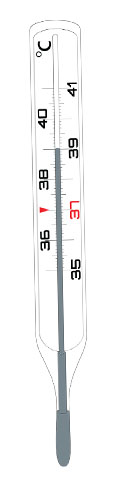
\includegraphics[width=1.1cm]{Images/nhietkethuyngan}
			& 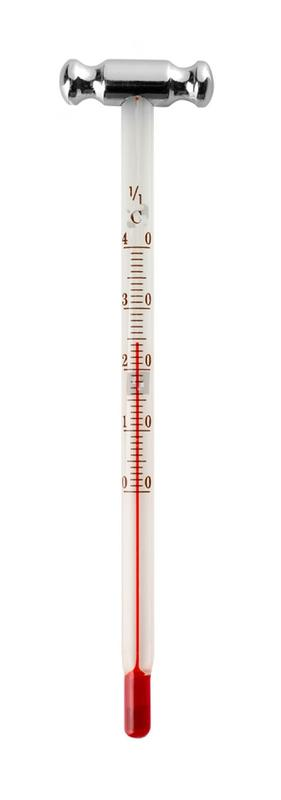
\includegraphics[width=1.4cm]{Images/nhietkeruou1}&  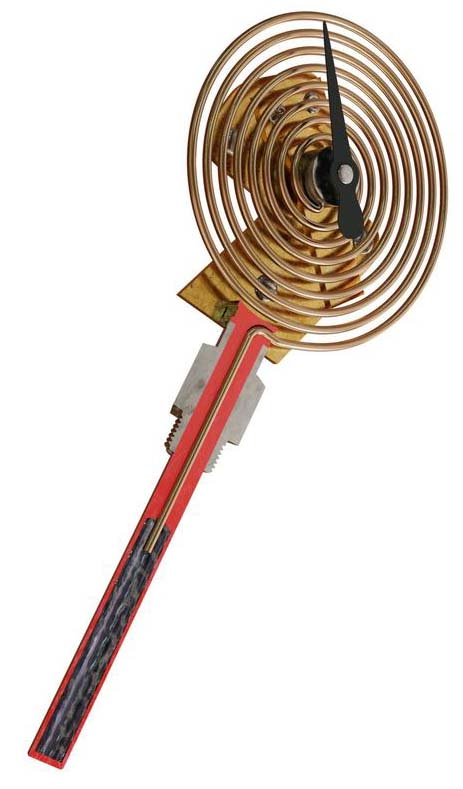
\includegraphics[width=2.3cm]{Images/nhietkekimloai}&  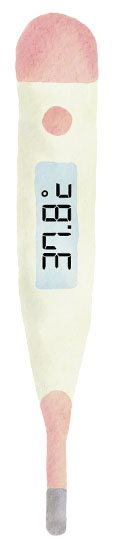
\includegraphics[width=0.9cm]{Images/nhietkeyte}\\
			\hline
			Dải nhiệt độ & $-10^\circ C$ đến $110^\circ C$ & $-30^ \circ C$ đến $60^\circ C$	
			& $0^\circ C$ đến $400^\circ C$ & $34^\circ C$ đến $42^\circ C$	
			\\
			\hline
		\end{tabular}
	\end{center}
	\choiceTF[t]
	{\True Dùng nhiệt kế kim loại để đo nhiệt độ của bàn là}
	{\True Dùng nhiệt kế y tế để đo nhiệt độ của cơ thể người}
	{\True Dùng nhiệt kế thủy ngân để đo nhiệt độ của nước đang sôi}
	{\True Dùng nhiệt kế rượu để đo nhiệt độ của không khí trong phòng}
	\loigiai{
		\begin{enumerate}[label=\alph*)]
			\item Đúng 
			\item Đúng
			\item Đúng
			\item Đúng
		\end{enumerate}
		
	}
	\haidong{4}\end{ex}
	